\documentclass[a4paper,sffamily,12pt]{article}

\usepackage[T1]{fontenc}
\usepackage[french]{babel}
\usepackage[utf8]{inputenc}

% Insertion d'image
\usepackage{graphicx}

% Création de lien
\usepackage[colorlinks,linkcolor=blue]{hyperref}

% Formatage des titres de sections
\usepackage{titlesec}
\titleformat{\section}
  {\normalfont\Large\bfseries\sffamily}{\thesection.}{0.33em}{}[\hrule]
\titleformat{\paragraph}
  {\normalfont\bfseries\sffamily}{\theparagraph.}{0.33em}{}
 
 % En-tête
\usepackage{fancyhdr}
\pagestyle{fancy}
\renewcommand\headrulewidth{1pt}
\fancyhead[L]{Base de données évoluées}
\fancyhead[R]{$X1I1050$}

% Permet de mettre du texte au dessus du titre
\usepackage{titling}
\renewcommand{\maketitlehooka}{\noindent COUILLEROT Carol \hfill \\ MAHIER Loïc \hfill \\ PHALAVANDISHVILI  Demetre}

% Titre
\title{\vspace{\fill}\LARGE\bfseries\sffamily Rapport de projet\protect\footnote{rapport réalisé sous \LaTeX} \vspace{\fill}}

\begin{document}

	\date{} % Supprime la date
	\maketitle % Affiche le titre

	\thispagestyle{fancy} % Permet de mettre le titre sur la page ''fancy''
	
	\newpage
			
	\renewcommand{\contentsname}{Sommaire}
	\tableofcontents
	
	\newpage
	
	\section{Introduction}

		\vspace{0.5cm}
		
		L'objectif de ce projet est de réaliser un entrepôt de données (OLAP) ainsi que des requêtes intéressantes sur un ou plusieurs jeu de données libres (open data). Pour ce faire nous avons choisis deux jeux de données : un sur les hébergements collectifs en France et l'autre sur les communes. Nous avons également choisis de réaliser ce projet en PL/SQL ainsi que d'utiliser Talend pour nettoyer nos données et concevoir nos tables relationnelles. \\

	\section{Choix des données}				

		\vspace{0.5cm}
		
		 Nous avons trouver nos données sur le site \url{https://public.opendatasoft.com/explore}, elles sont également présente sur le site \url{https://www.data.gouv.fr}. Le premier jeu de données est sur les hébergements collectifs en France : c'est à dire les hôtels, les campings et les résidences avec des informations sur leur location, leur classement (nombre d'étoile) et leur capacité d'accueil notamment. Le deuxième jeu de donnée recueil toutes les communes de France, en indiquant leur population, leur superficie, leur code postal ainsi que leur département et leur région entre autre. Ce dernier nous permet d'affiner nos requête, d'en proposer des plus complexes mais aussi de pouvoir faire des regroupements et des classements par région et par département. Nous allons ainsi pouvoir faire des requêtes sur le classement (nombre d'étoile) de ces hébergements par département et région. Nous pourrons aussi regarder par commune, le nombre d'hôtels par habitant ou bien même faire une comparaison du nombre d'hébergement par région en fonction de l'année. \\

		\vspace{0.5cm}
		
	\section{Constellation de fait}

		\vspace{0.5cm}
			
		Après avoir choisis nos jeux de données, nous avons décidé de distinguer deux tables de faits : une propre aux hébergements avec des informations sur leur capacité d'accueil et leur classement par exemple. Et une seconde propre aux communes, avec leur population, leur superficie et leur location (département, région). Quatre dimensions s'y ajoutent : une pour les date, une pour les adresses des hébergement, une pour les informations complémentaires des hébergements et enfin une relative aux communes avec un certain nombre de leur caractéristiques. Pour pouvoir faire des requêtes intéressantes et donc pour pouvoir joindre nos deux tables de faits, nous utilisons l'identifiant de l'hébergement qui est présent dans les deux tables de faits. Cela nous permet ainsi d'accéder aux caractéristiques propres à l'hébergement ainsi que celles propres à la commune de cette hébergement. \\
		
		Pour des raisons pratiques nous avons également choisis de faire une vue précise sur la location. Celle-ci nous affiche pour chaque commune, son code postale, son code INSEE, son département et sa région. Le code INSEE est essentiel puisqu'il est unique, en effet ils se trouve que plusieurs communes ont le même code postale. Cette vue simplifiera nos requêtes complexes, d'autant que nous l'utiliserons fréquemment. \\
	
		\vspace{0.5cm}
		
		\begin{figure}[!h]
				
			\centerline{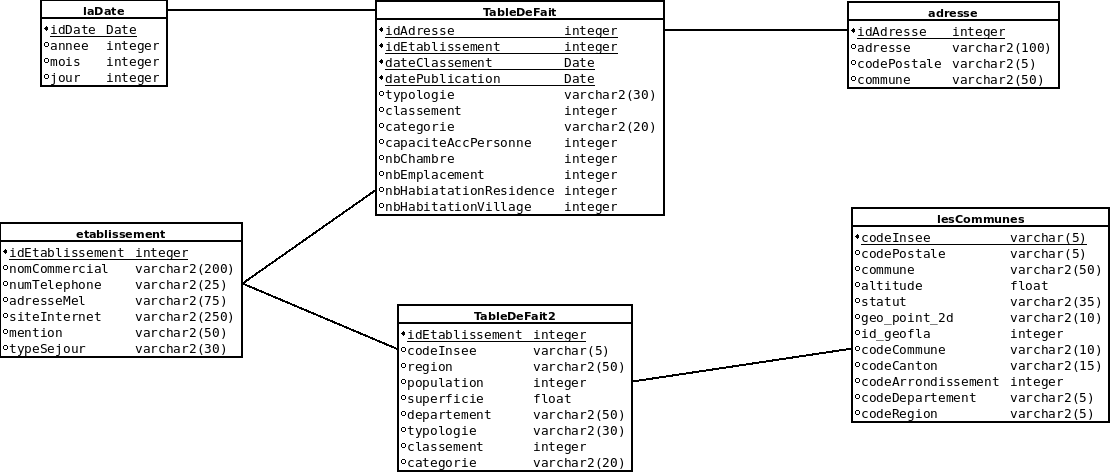
\includegraphics[height=8cm]{picture/constellation_de_fait.png}}
			\caption{La constellation de fait qui structure notre entrepôt de données}
			\label{constellation}
			
		\end{figure}	
		
		\vspace{0.5cm}
				
	\section{Intégration avec Talend}

		\vspace{0.5cm}
		
		Après avoir défini notre constellation de fait, notre prochain objectif était de commencer à intégrer nos jeux de données. Pour cela nous avons utiliser le logiciel Talend permettant de transformer nos données brut vers les tables relationnelles de la base de données Oracle. Pour réaliser cette transformation nous avons eu plusieurs étapes intermédiaires. La première étape consistait à lire le fichier au format ''.csv'' et à le décomposer en plusieurs tables conforment au schéma de fait définit dans la partie précédente. Pour cette décomposition nous avons utilisé à plusieurs reprises la fonction interne du logiciel Talend tMap. \\
		
    		\indent Le premier point important de l’utilisation de Talend était la création de la table laDate. En effet, dans notre premier jeu de données nous avons deux attributs de type date (datePublication et dateClassement). En utilisant les fonctions tUnite et tUniqRow de Talend, nous obtenons des dates uniques qu’on met dans la table laDate en ajoutant les attributs calculés année, mois et jour. \\
    		
    		\indent Le deuxième point important de l’utilisation de Talend est la création de la table lesCommunes, pour laquelle nous avons besoin d’utiliser les deux jeux de données pour faire l’intersection des codes postaux. Pour cela nous avons utiliser tUniqrow afin d'obtenir des communes uniques à partir du premier jeu de donnés, puis nous avons fait l’intersection avec le deuxième jeu de données en utilisant tMap. \\
    		
    		\indent Le troisième point important de l’utilisation de Talend est l’intégration des données nettoyées avec tMap dans la base de données Oracle. Pour cela nous avons utiliser la fonction tOracleOutput permettant d'insérer et de modifier les données à partir des tables définies dans tMap. Une fois configuré l’accès à la base de données, on précise les noms des tables (initialement vide) dans la base de données et enfin on obtient la base de données remplie des informations sur Oracle. \\		
		
		\vspace{0.5cm}
			
	\section{Requêtes d'analyses}

		\vspace{0.5cm}
		
		Une fois nos données sur Oracle, nous avons réalisé une dizaine de requête d'analyse en PL/SQL. Nous avons d'abord fait quelques requêtes sur la première table de fait, puis sur la deuxième avant d'en concevoir des plus complexes englobant les deux tables. Pour ces requêtes nous avons essayé de réutiliser un grand nombre d'extension de SQL tels que ROLLUP, CUBE et GROUPING SET notamment. \\		
		
		Pour ce faire, nous avons identifié différents acteurs qui pourraient être amené à utiliser ce jeu de données, par exemple les collectivités, un client lambda et un promoteur. Et c'est en nous mettant à leur place que l'on a essayé de faire le tour d'horizon des requêtes utiles : ainsi un client pourrait souhaiter savoir quel est le meilleur hôtel dans le département ou la région de ses vacance. De même un promoteur cherchant à bâtir un nouvelle établissement (hôtel, résidence, camping, ...) aimerait savoir quel département est en manque d'hébergement. Ainsi on peut imaginer différent type de requête, les unes tournées vers l'analyse ''touristique'' informant sur le classement, le meilleur service, la proximité et les autres tournées sur l'analyse de ''couverture'', informant ainsi davantage sur la quantité d'hébergement dans une zone, la capacité d'accueil des hôtels ans une ville , etc. \\
		
		Aussi, nous avons jugé utile de créer quelques vues, notamment une faisant la jointure entre les adresses de nos hébergements et la dimensions lesCommunes, ce qui simplifie nos requêtes. Nous avons également fait des vues pour avoir de pré-calculé toutes les sommes ou moyennes qui pourraient nous servir dans nos requête. Enfin nous avons choisi d'indexer quelque attribut souvent appelé à l'aide d'index bitmap. \\
		
		\vspace{0.5cm}
																
	\section{Conclusion}

		\vspace{0.5cm}
		
		Ainsi, nous avons réussi à créer notre premier entrepôt de donnée. Nous avons également réussi à proposer des requêtes pertinentes, analysant bien nos données. Ce projet nous aura permis de nous familiariser davantage avec les extensions de SQL tels que ROLLUP et CUBE notamment. La partie la plus ardue aura finalement été l'intégration des données avec Talend qui est un logiciel assez difficile à prendre en main mais au final extrêmement pratique et puissant. L'intégration ayant été faites sur Talend, tout en sachant que l'on peut directement envoyer nos données sur Oracle depuis Talend, il serait donc assez facile aujourd'hui d'ajouter de nouveaux jeux de données à notre entrepôt pour étendre notre champs d'analyse ou l'affiner encore davantage. \\
						
\end{document}
